The concluding chapter explores the system implementation details, clarifying the integration of its components and delineating the methodologies employed for validation and verification. \\
In light of this, the implemented testing protocols' primary objective is to fix most application bugs before each release, recognizing the intrinsic challenge of eliminating all defects. Therefore, while the initial paragraph focuses on the complexities of the implementation strategy, expected consideration is given to the integration test plan during its formulation. \\
Emphasizing the significance of comprehensive documentation, the code is expected to be well-commented and meticulously documented, utilizing tools such as Javadoc to extend the documentation process, ensuring clarity and facilitating a deeper understanding of the codebase. This approach to implementation, integration, and documentation aims to enhance the robustness and maintainability of the CodeKataBattle platform. \\ \\

\subsection{Implementation plan}
The implementation approach for the CodeKataBattle platform blends the advantages of bottom-up and thread strategies, ensuring a comprehensive and effective development process. Adopting a threading strategy permits the generation of intermediate deliverables, providing stakeholders with measurable milestones crucial for validating the evolving system. Concurrently, employing a bottom-up strategy promotes incremental integration, boosting efficient bug tracking through the iterative testing of intermediate versions and the subsystems resulting from the integration of components.

The thread strategy entails a meticulous identification of system features and the corresponding portions of components (referred to as sub-components for practicality) responsible for delivering these features. A single function often involves collaboration among different sub-components, and a strategic order for their implementation is essential. The bottom-up approach is incorporated to address this challenge.

This implementation strategy facilitates the parallel assignment of feature implementation tasks to independent development teams, enabling concurrent progress. However, before this allocation, it is imperative to identify any common components to prevent redundant efforts in producing the same component or subcomponent. This hybrid approach, amalgamating bottom-up and thread strategies, is balanced to simplify the development process, improve collaboration among development teams, and optimize the overall implementation of the CodeKataBattle platform.

These processes provide incremental development, stakeholder engagement, bug tracking and testing, parallel development, adaptability to complexity, and avoidance of redundancy fitting perfectly the CodeKataBattle platform's needs.

Before proceeding with the component integration and testing paragraph, it can be useful to identify the features of the system starting from the requirements themselves.
\begin{itemize}
    \item \textbf{[F1] User registration and authentication:} \\
    User registration and authentication are entangled functionalities, each playing a role in ensuring secure access to the CodeKataBattle platform. Considering these features together is crucial, as the authentication process necessitates prior registration.
    During this phase, it is vital to establish a clear distinction between student and educator profiles. The system must store these distinct account types allowing for future distinguishability. This delineation ensures that, depending on whether a user is logged in as an educator or a student, the system provides dedicated commands and privileges tailored to the respective roles. This careful segregation improves the user experience, aligning the platform with the specific needs and permissions associated with each account type.
    
    \item \textbf{[F2] Tournament creation:} \\
    Tournament creation is a feature exclusive to educators. Only educators can initiate tournaments, utilizing purpose-built interfaces to articulate essential details such as the description and rules. This separation of authority ensures that the responsibility of shaping the tournament landscape aligns with the instructional role of educators, facilitating a streamlined and organized creation process.
    
    \item \textbf{[F3] Battle creation:} \\
    Educators can craft code kata battles within tournaments: the process consists of uploading code katas, defining group size constraints, establishing registration and submission deadlines, and configuring scoring parameters. It's important that within a given tournament, multiple educators may contribute by creating battles. However, an essential check is embedded in the system to ensure that educators seeking to create battles within the same tournament have obtained prior authorization from the tournament's creator. This measure maintains a structured and collaborative environment, aligning with the platform's governance model.
    
    \item \textbf{[F4] Allow other educators to crate battles:} \\
    Involving additional educators in the creation of battles within a tournament implicates a systematic invitation process facilitated through a dedicated interface. This step is exclusively within the privileges of the tournament creator.
    
    \item \textbf{[F5] Student registration to tournament and battle, Team formation:} \\
    Upon logging into the platform, students can register for tournaments through a dedicated function. Once enrolled in one or more tournaments, students can further register and actively participate in the battles associated with those tournaments. A key aspect of the software development process lies in the concurrent consideration of team formation and battle registration. Team formation develops immediately after the registration process, inviting additional students through a specialized form.
    The team registration must be completed before the registration deadline expires. Only when the team reaches a valid number of members, it transitions to active participation in the battle. This set of sequential events and requisite conditions highlights the intrinsic connection between these features, requiring a comprehensive and cohesive testing approach that evaluates their combined functionality.
    
    \item \textbf{[F6] GitHub Integration:} \\
    The integration with GitHub is necessary for the correct functioning of the platform. This integration plays a dual role: the system relies on it for the accurate creation of a battle, while students leverage it to configure GitHub Actions, automating the code submission process to the platform. This collaborative interaction ensures the synchronization of platform operations and student workflows, reinforcing the platform's robust and efficient code submission mechanism. 
    
    \item \textbf{[F7] Manual evaluation:} \\
    This feature authorizes educators with the ability to manually evaluate student code, in addition to automated evaluation, before final rankings are determined.
    
    \item \textbf{[F8] Tournament closure:} \\
    Educators can decide to manually close the tournament. The tournament closure requires several integrity checks that must be performed by many components.
   
    \item \textbf{[F9] Badge creation and assignment:} \\
    After educators have created a tournament, they can augment gamification by adding badges through dedicated interfaces. Within this process, educators utilize a specific language to articulate the constraints that define the conditions under which a student can earn these badges. When the tournament is closed, the badges are automatically assigned to deserving students. 
    
    \item \textbf{[F10] Notification system:} \\
    Whenever a tournament or a battle undergoes a state change, users directly involved receive notifications containing all pertinent information to guide them through the game. The notification system is also integrated with the login process, educator invitation process, and team formation process.
    
\end{itemize}

\subsection{Component integration and testing}

The integration of components takes place following the implementation of features. Once all the components contributing to a specific feature are individually implemented, they are tested in conjunction with the functionalities they collectively represent. This systematic integration approach ensures that features are not only implemented on an individual basis but are also rigorously assessed for collaborative functionality.

\begin{itemize}
    \item \textbf{[F1] User registration and authentication:} \\
        The highest priority lies in the implementation and testing of registration and authentication functionalities since nearly every other system function necessitates user authorization and logging (as described in \ref{fig:T_F1}).
        
        \begin{figure}[h!]
            \centering
            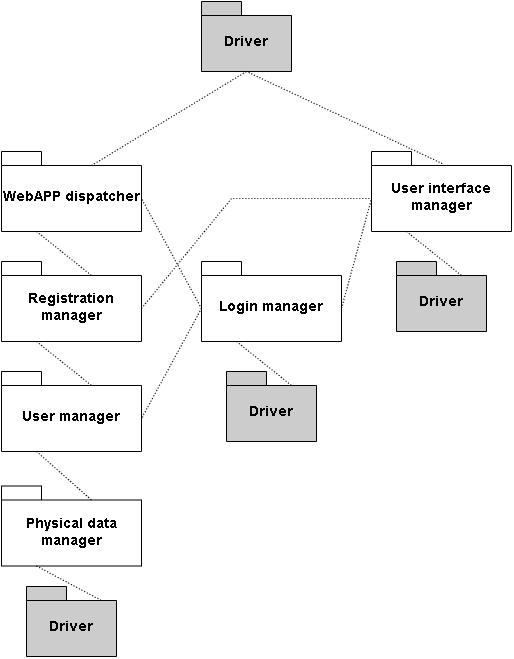
\includegraphics[width=\linewidth]{Images/T_F1.png}
            \caption{F1 Developing}
            \label{fig:T_F1}
        \end{figure}

    \item \textbf{[F2] Tournament creation:} \\
        Next in line are the tournament creation functionalities, crucial to developing battles and supporting all the intricate functionalities within the game (as described in \ref{fig:T_F2}).
    
        \begin{figure}[h!]
            \centering
            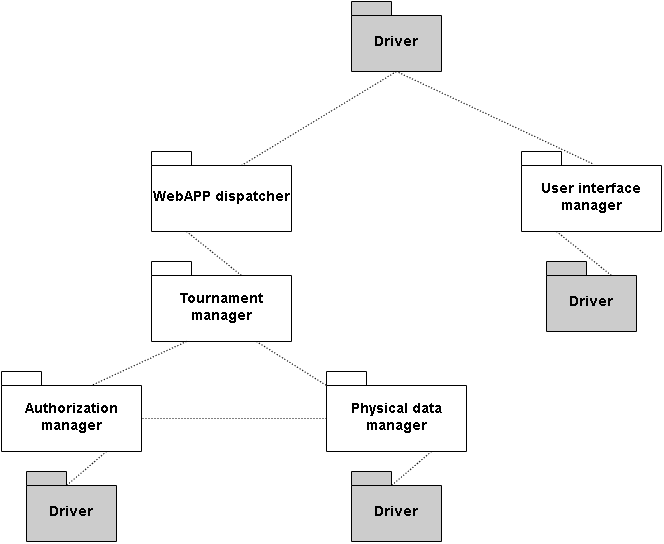
\includegraphics[width=\linewidth]{Images/T_F2.png}
            \caption{F2 Developing}
            \label{fig:T_F2}
        \end{figure}
    
    \item \textbf{[F3] Battle creation:} \\
        To complete the basic functionalities of the platform we need to implement and test F3 (as described in \ref{fig:T_F3}). \\
        
        \begin{figure}[h!]
            \centering
            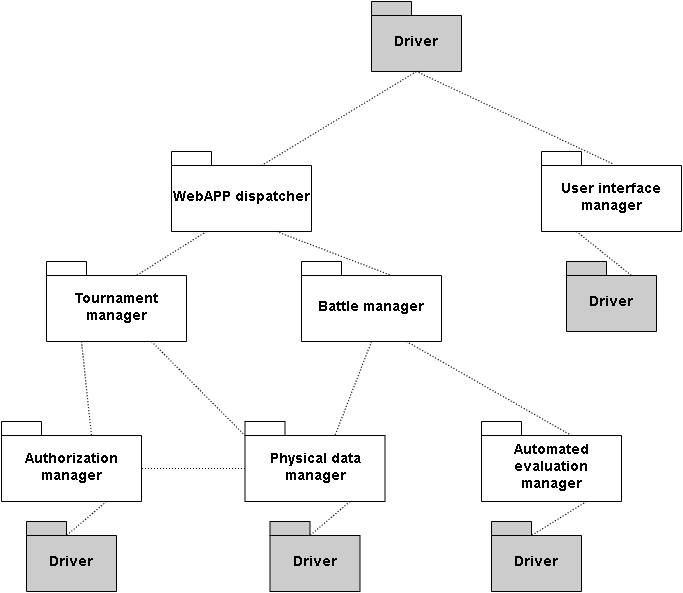
\includegraphics[width=\linewidth]{Images/T_F3.png}
            \caption{F3 Developing}
            \label{fig:T_F3}
        \end{figure}

\end{itemize}
    
Once the features F1, F2, and F3 are created and validated, the platform's fundamental building blocks are in place. The following functionalities can be implemented concurrently without a specific sequence, promoting a parallel development and testing process. This approach accelerates the system's production by allowing teams to work on different aspects.

\begin{itemize}

    \item \textbf{[F4] Allow other educators to crate battles:} \\
        The developing structure is described in the \ref{fig:T_F3}.
    \item \textbf{[F5] Student registration to tournament and battle, Team formation:} \\
        The developing structure is described in the \ref{fig:T_F3} and \ref{fig:T_F2}.
        
    \item \textbf{[F6] GitHub Integration:} \\
        In \ref{fig:T_F6} is visible that we only need to add the GitHub Integration Manager component to implement this feature.
        \begin{figure}[h!]
            \centering
            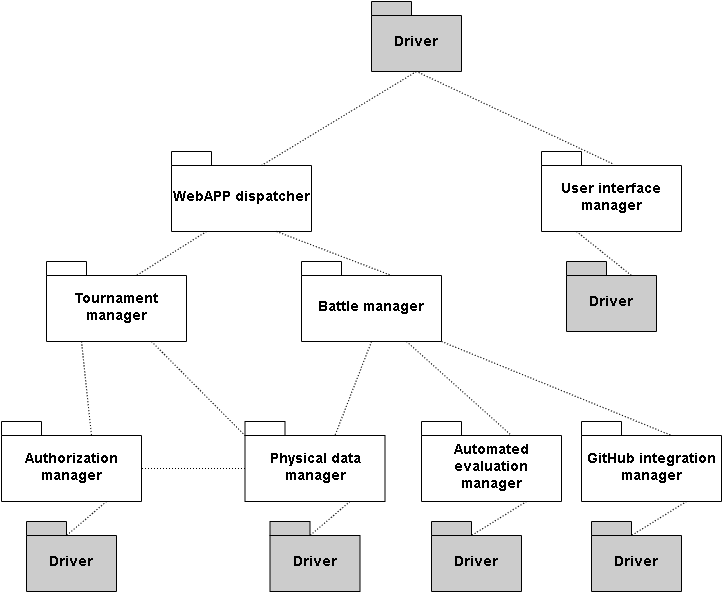
\includegraphics[width=\linewidth]{Images/T_F6.png}
            \caption{F6 Developing}
            \label{fig:T_F6}
        \end{figure}
    
    \item \textbf{[F7] Manual evaluation:} \\
        The developing structure is described in the \ref{fig:T_F3} and \ref{fig:T_F2}.
    \item \textbf{[F8] Tournament closure:} \\
        The developing structure is described in the \ref{fig:T_F3} and \ref{fig:T_F2}.
        
    \item \textbf{[F9] Badge creation and assignment:} \\
        In order to implement and test F9 we need to properly integrate the Badge Manager as described in \ref{fig:T_F9}.
        \begin{figure}[h!]
            \centering
            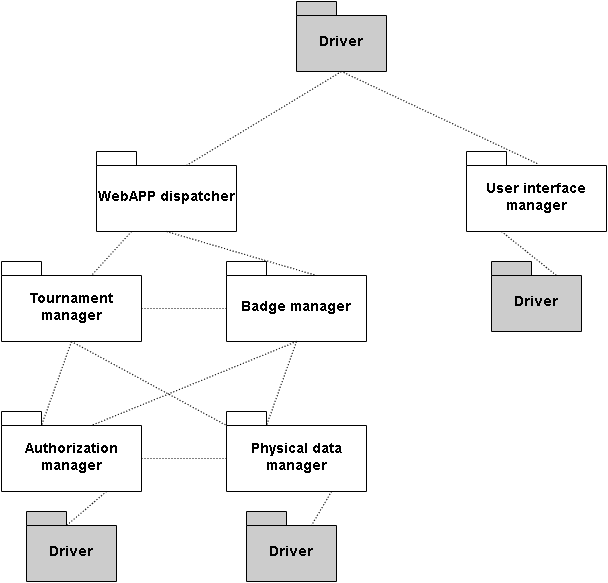
\includegraphics[width=\linewidth]{Images/T_F9.png}
            \caption{F9 Developing}
            \label{fig:T_F9}
        \end{figure}
        
    \item \textbf{[F10] Notification system:} \\
    To conclude the implementation phase, the final component to be developed is the notification system. This element needs to be integrated with all components that directly communicate with users through push notifications or emails  (see \ref{fig:T_F10}).
        \begin{figure}[H]
            \centering
            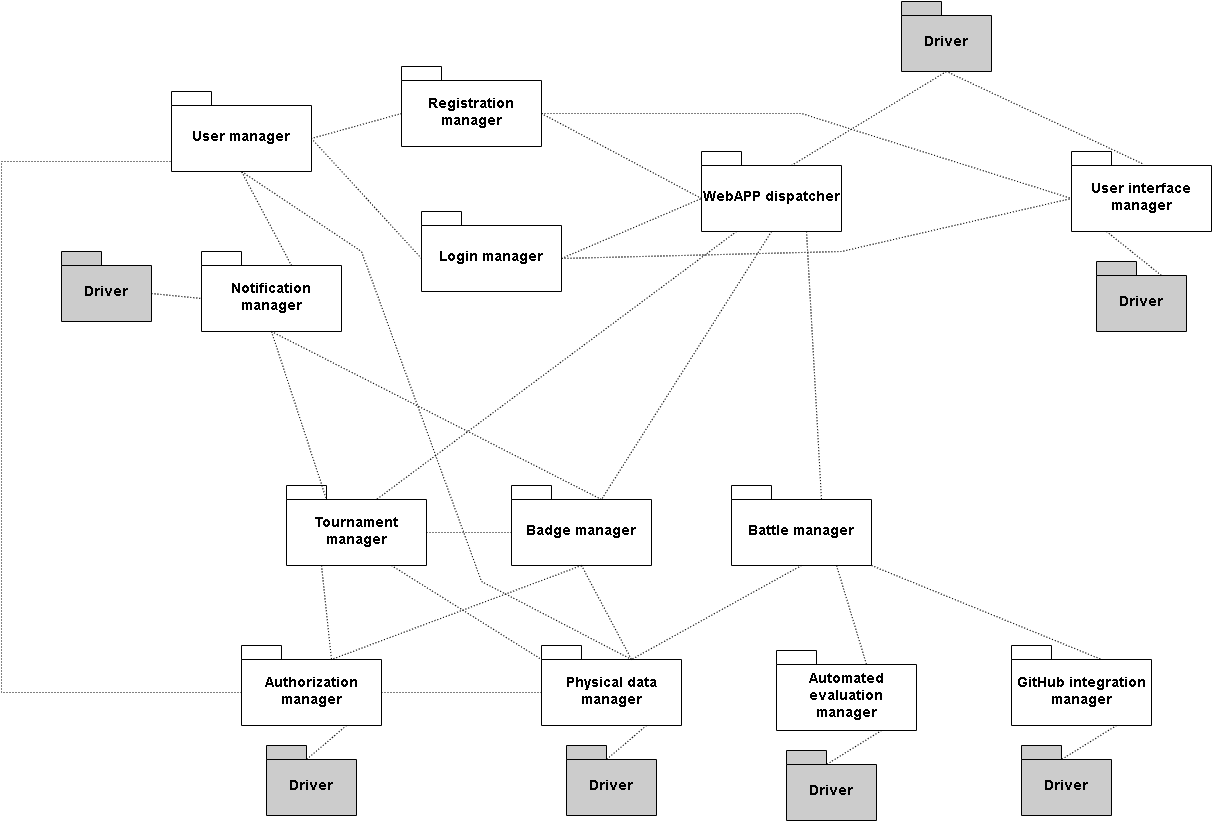
\includegraphics[width=\linewidth]{Images/T_F10.png}
            \caption{F10 Developing}
            \label{fig:T_F10}
        \end{figure}
    
\end{itemize}


\newpage

\subsection{System testing}

The CodeKataBattle platform undergoes systematic testing, considering various levels of granularity and scopes to ensure the reliability and functionality of its components. In the development phase, individual modules and components go through unit testing in isolation to verify their expected performance. To facilitate this, the creation of Driver and Stub components simulates the behavior of surrounding modules, considering both expected and unexpected scenarios to evaluate robustness.

Subsequently, the integration and testing phase employs bottom-up and thread strategies, aligning with the platform's architectural design. As components are integrated, the focus shifts to validating their collaborative functioning. Once individual components and their integrations have been tested and fixed, the system testing begins to validate adherence to functional and nonfunctional requirements outlined in the RASD.

The system testing phase includes:
\begin{itemize}
    \item \textit{Functional Testing:} Ensuring the system meets all specified requirements from the RASD. This phase may also expose opportunities to improve user experience with new features.
    \item \textit{Performance Testing:} Identifying potential bottlenecks, inefficient algorithms, and other performance-related issues that could affect the system's responsiveness, utilization, and throughput. This phase requires an expected workload and predefined performance targets.
    \item \textit{Usability Testing:} Evaluating how well users can interact with the web application to accomplish tasks. Given the platform's emphasis on user-friendly design, usability testing is essential.
    \item \textit{Load Testing:} Uncovering bugs such as memory leaks or mismanagement and determining the upper limits of system components. It involves gradually increasing the load until reaching the system's operational threshold.
    \item \textit{Stress Testing:} Ensuring agile system recovery after failure by intentionally subjecting it to overwhelming resource demands or deprivation.
\end{itemize}

This testing approach ensures the CodeKataBattle platform's robustness, performance, and user-centric design across various scenarios and usage conditions. It also provides a workflow for continuous improvement and advancement based on testing outcomes.